
% \documentclass[acmtog, nonacm]{acmart}
\documentclass[sigconf, nonacm]{acmart}

% Suppress all metadata, footnotes, and contact blocks
\makeatletter
\renewcommand{\@acmVolume}{}
\renewcommand{\@acmNumber}{}
\renewcommand{\@acmArticle}{}
\renewcommand{\@acmYear}{}
\renewcommand{\@acmMonth}{}
\renewcommand{\@acmDOI}{}
\renewcommand{\@copyrightpermission}{}
\renewcommand{\@seriesname}{}
\renewcommand{\@acmPrice}{}
\renewcommand{\@authorsaddresses}{} % Remove authors' contact info
\renewcommand{\@authornotemark}{}   % Remove author contribution notes
\patchcmd{\maketitle}{\@typesetauthors}{\relax}{}{} % Remove footnote markers
\makeatother

% Remove ACM reference format and blocks
\settopmatter{printacmref=false, printccs=false, printkeywords=false}
\renewcommand\footnotetextcopyrightpermission[1]{} % Suppress footer

\pagestyle{plain}
\usepackage{enumitem}
\setlist[itemize]{leftmargin=12pt}
\setlist[enumerate]{leftmargin=*}
\usepackage{hyperref}
\usepackage{graphicx}
\usepackage{booktabs}
\usepackage{multirow}
\usepackage{amsmath}
\usepackage{amssymb}

% Space-saving measures to fit within 8 pages
\setlength{\textfloatsep}{8pt plus 2pt minus 2pt}
\setlength{\floatsep}{8pt plus 2pt minus 2pt}
\setlength{\intextsep}{8pt plus 2pt minus 2pt}

\begin{document}

%%
%% The "title" command has an optional parameter,
%% allowing the author to define a "short title" to be used in page headers.
\title{Traffic Safety: Analyzing Crash Inequality Across Chicago Neighborhoods Using Machine Learning and Network Science}

%%
%% The "author" command and its associated commands are used to define
%% the authors and their affiliations.

\author{Siddarth Bandi}
\affiliation{%
  \institution{Virginia Tech}
  \department{Computer Science}
  \city{Alexandria, VA}
  \country{USA}}
\email{siddarth24@vt.edu}

\author{Shubam Khantwal}
\affiliation{%
  \institution{Virginia Tech}
  \department{Computer Science}
  \city{Alexandria, VA}
  \country{USA}}
\email{shubam@vt.edu}


\author{Venkata Sai Yaswanth Madiraju}
\affiliation{%
  \institution{Virginia Tech}
  \department{Computer Science}
  \city{Alexandria, VA}
  \country{USA}}
\email{yaswanth1@vt.edu}

\renewcommand{\shortauthors}{}

%%
%% The abstract is a short summary of the work to be presented in the
%% article.
\begin{abstract}
Traffic crashes remain a critical public safety concern in urban environments, yet their distribution across communities is far from uniform. This study analyzes traffic crash inequality across Chicago's 78 community areas using machine learning, network science, and spatial statistics to predict future crash hotspots and assess socioeconomic disparities in crash exposure. We developed a temporally-validated Gradient Boosting model that achieved PR-AUC of 0.772 and ROC-AUC of 0.946 in predicting future crash hotspots at 19,200 intersections using 1.0 million historical crash records (2013-2025). Historical crash frequency emerged as the dominant predictor (90\% feature importance), followed by network centrality measures and demographic factors. Our inequality analysis revealed significant disparities: lower-income communities experience 80\% higher severe injury rates compared to high-income areas (correlation: r=-0.488, p<0.001). Spatial autocorrelation analysis (Moran's I = 0.161, p<0.001) confirmed that crashes cluster geographically rather than occurring randomly. Local Moran's I (LISA) identified 964 High-High cluster intersections requiring immediate intervention. The model successfully identified 1,875 persistent hotspots and 457 emerging hotspots for proactive intervention, demonstrating the utility of data-driven approaches for equitable urban safety policy.
\end{abstract}

%%
%% This command processes the author and affiliation and title
%% information and builds the first part of the formatted document.
\maketitle

\section*{\textbf{Keywords}}
\textbf{Urban Computing, Traffic Safety, Crash Prediction, Machine Learning, Network Science, Spatial Statistics, Inequality Analysis, Temporal Validation, Gradient Boosting, LISA Clustering}

\section{Introduction}

Traffic crashes are a leading cause of injury and death in urban areas, with profound implications for public health, economic productivity, and social equity. In the United States, traffic crashes cost over \$340 billion annually and result in approximately 38,000 deaths each year \cite{nhtsa2021}. However, the burden of traffic crashes is not distributed equally across urban communities. Certain intersections and neighborhoods experience disproportionately high crash rates, often correlating with socioeconomic factors such as income, vehicle ownership, and infrastructure quality.

Chicago, the third-largest city in the United States, provides an ideal testbed for studying traffic crash inequality. The city's 78 distinct community areas exhibit significant demographic diversity and infrastructure variation. Understanding which intersections will become future crash hotspots—and why certain communities bear a greater crash burden—is essential for policymakers to design evidence-based interventions, allocate resources equitably, and advance Vision Zero goals.

\subsection{Problem Statement}

This study addresses three interconnected research questions: (1) \textit{Can machine learning models accurately predict which intersections will become future crash hotspots?} (2) \textit{Are crashes and severe injuries distributed equally across Chicago's neighborhoods, or do certain communities bear a disproportionate burden?} and (3) \textit{Do crashes exhibit spatial clustering patterns that justify geographically-targeted interventions?}

\subsection{Our Approach}

We employ a multi-faceted urban computing approach combining: (1) \textbf{Machine learning} for predictive modeling using temporally-validated classification, (2) \textbf{Network science} to analyze the role of road network structure via centrality measures, and (3) \textbf{Spatial statistics} using Moran's I and LISA clustering to detect geographic patterns. Our dataset integrates 1,001,020 crash records from the Chicago Data Portal, OpenStreetMap road network data, and U.S. Census demographics.

\subsection{Contributions}

Our key contributions include:
\begin{itemize}
    \item A \textbf{temporally-validated predictive model} achieving PR-AUC of 0.772 for identifying future crash hotspots, using proper chronological train/test splits to prevent data leakage
    \item \textbf{Evidence of crash inequality}: lower-income communities experience significantly higher severe injury rates (r=-0.488, p<0.001)
    \item \textbf{Spatial clustering confirmation}: crashes exhibit significant positive autocorrelation (Moran's I = 0.161, p<0.001), with 964 High-High cluster intersections identified
    \item \textbf{Actionable insights}: identification of 1,875 persistent hotspots requiring immediate intervention and 457 emerging hotspots for proactive measures
    \item A \textbf{reproducible open-source pipeline} for crash prediction and inequality analysis applicable to other cities
\end{itemize}

\section{Related Work}

\subsection{Traffic Crash Prediction}

Machine learning has been extensively applied to traffic safety analysis. Chen et al. \cite{chen2016crash} used random forests to predict crash severity, achieving 75\% accuracy but relying on random train/test splits that risk data leakage. Gutierrez-Osorio and Pedraza \cite{gutierrez2020modern} surveyed deep learning approaches for crash prediction, highlighting CNNs and RNNs for spatiotemporal modeling. However, most studies focus on crash severity classification rather than proactive hotspot identification.

Bao et al. \cite{bao2020spatial} applied gradient boosting to predict crash frequency at signalized intersections, identifying traffic volume and geometric features as key predictors. Our work extends this by incorporating network centrality measures and demographic factors, while using rigorous temporal validation.

\subsection{Spatial Analysis of Crashes}

Spatial clustering methods have proven effective for hotspot detection. Plug et al. \cite{plug2011spatial} used kernel density estimation to identify crash hotspots in the Netherlands, while Prasannakumar et al. \cite{prasannakumar2011spatial} applied Getis-Ord Gi* statistics for hotspot mapping in India. 

Moran's I and LISA (Local Indicators of Spatial Association) have been applied to crime \cite{anselin1995local} and disease clustering \cite{jacquez2005spatial}, but their application to traffic safety remains limited. Our work systematically applies both global and local Moran's I to quantify spatial autocorrelation and identify specific cluster types (High-High, Low-Low, etc.).

\subsection{Network Science in Traffic Safety}

Network science approaches have emerged for understanding crash patterns. Xu et al. \cite{xu2013network} analyzed crash networks in urban areas, finding that high-betweenness intersections experience more crashes. Kerner et al. \cite{kerner2015traffic} demonstrated that network congestion patterns influence crash risk.

Our work integrates degree, closeness, and betweenness centrality as predictive features, explicitly testing whether network topology contributes to crash prediction beyond historical crash counts.

\subsection{Crash Inequality and Environmental Justice}

Recent studies have documented disparities in crash exposure. Cottrill and Thakuriah \cite{cottrill2010evaluating} found that low-income communities in Chicago experience higher pedestrian crash rates. Beck et al. \cite{beck2007motor} showed that motor vehicle crash death rates are inversely correlated with income at the census tract level.

However, these studies are largely descriptive. Our work advances the field by: (1) integrating inequality analysis with predictive modeling, (2) using spatial statistics to confirm clustering patterns, and (3) providing actionable hotspot prioritization for equitable resource allocation.

\section{Algorithms and Methodology}

\subsection{Data Collection and Integration}

We integrated data from four primary sources to construct a comprehensive spatiotemporal dataset:

\begin{itemize}
    \item \textbf{Chicago Traffic Crashes - Crashes}: 1,001,020 crash records (2013-2025) from the Chicago Data Portal, including location, timestamp, and severity
    \item \textbf{Chicago Traffic Crashes - People}: 167,943 injury records with detailed injury classifications
    \item \textbf{OpenStreetMap}: Chicago road network with 29,366 nodes and 65,000+ edges
    \item \textbf{U.S. Census (ACS)}: Demographics for 78 community areas including median income, population, and vehicle ownership
\end{itemize}

\subsection{Preprocessing Pipeline}

\textbf{Spatial Matching}: We matched crashes to the nearest OpenStreetMap intersection node using geodesic distance calculations in a projected coordinate system (EPSG:26971 - NAD83 Illinois East). This achieved an 88\% match rate, linking 880,457 crashes to 19,200 unique intersections.

\textbf{Temporal Feature Engineering}: We constructed features using rolling time windows to enable temporal validation (Figure~\ref{fig:temporal_windows}):

\begin{itemize}
    \item \textbf{Historical window} (365 days before cutoff): Features for prediction
    \item \textbf{Recent window} (90 days before cutoff): Short-term trend features
    \item \textbf{Future window} (180 days after cutoff): Labels for hotspot classification
\end{itemize}

For each intersection and time period, we computed:
\begin{equation}
    \text{hist\_crashes}_i = \sum_{t \in [t_0 - 365d, t_0]} \mathbb{1}\{\text{crash at node } i \text{ at time } t\}
\end{equation}

\begin{equation}
    \text{hist\_severity}_i = \sum_{t \in [t_0 - 365d, t_0]} w(\text{severity}_t)
\end{equation}

where severity weights are: Fatal=5, Incapacitating=4, Non-incapacitating=3, Reported=2, No injury=1.

\begin{figure}[t]
    \centering
    \includegraphics[width=0.42\textwidth]{temporal_windows_diagram.png}
    \caption{Temporal feature engineering strategy showing historical (365 days), recent (90 days), and future (180 days) windows. The cutoff date slides forward every 6 months to create 23 time periods for proper temporal validation.}
    \label{fig:temporal_windows}
\end{figure}

\subsection{Network Centrality Features}

We computed three network centrality measures using NetworkX:

\textbf{Degree Centrality}: Number of roads connecting to an intersection, normalized by network size:
\begin{equation}
    C_D(i) = \frac{k_i}{n - 1}
\end{equation}
where $k_i$ is the degree of node $i$ and $n$ is the total number of nodes.

\textbf{Betweenness Centrality}: Fraction of shortest paths passing through node $i$:
\begin{equation}
    C_B(i) = \sum_{s \neq i \neq t} \frac{\sigma_{st}(i)}{\sigma_{st}}
\end{equation}
where $\sigma_{st}$ is the number of shortest paths from $s$ to $t$, and $\sigma_{st}(i)$ is the number passing through $i$.

\textbf{Closeness Centrality}: Inverse of average shortest path length to all other nodes:
\begin{equation}
    C_C(i) = \frac{n-1}{\sum_{j \neq i} d(i,j)}
\end{equation}

These features capture the hypothesis that high-traffic intersections (high centrality) experience more crashes due to increased vehicle exposure.

\subsection{Hotspot Label Definition}

We define hotspots as the top 10\% of intersections by future crash count within each time period:
\begin{equation}
    y_i = \begin{cases}
        1 & \text{if } \text{future\_crashes}_i \geq \text{quantile}_{0.90} \\
        0 & \text{otherwise}
    \end{cases}
\end{equation}

This threshold balances resource constraints (cities cannot fix all intersections) with capturing high-risk locations.

\subsection{Temporal Validation Strategy}

To prevent data leakage, we implement \textbf{chronological splitting} rather than random partitioning. We generate 23 time periods by sliding the cutoff date every 6 months from June 2014 to April 2025, creating 399,073 intersection-time samples.

\begin{itemize}
    \item \textbf{Train}: 70\% earliest periods (2014-06 to 2021-10): 248,913 samples
    \item \textbf{Validation}: 15\% middle periods (2022-04 to 2023-04): 64,401 samples
    \item \textbf{Test}: 15\% recent periods (2023-10 to 2025-04): 85,759 samples
\end{itemize}

This simulates real-world deployment where models trained on historical data must predict future events. We verify temporal integrity by ensuring no overlap:
\begin{equation}
    t_{\text{train}}^{\text{end}} < t_{\text{val}}^{\text{start}} < t_{\text{val}}^{\text{end}} < t_{\text{test}}^{\text{start}}
\end{equation}

\subsection{Machine Learning Models}

We evaluate three classification algorithms:

\textbf{Logistic Regression} (baseline): Linear model with L2 regularization and class balancing:
\begin{equation}
    P(y=1|x) = \frac{1}{1 + e^{-(\beta_0 + \beta^T x)}}
\end{equation}

\textbf{Random Forest}: Ensemble of 300 decision trees with balanced class weights and unlimited depth. Trees are trained on bootstrap samples with random feature subsets.

\textbf{Gradient Boosting}: Sequential ensemble building trees to minimize residual loss:
\begin{equation}
    F_m(x) = F_{m-1}(x) + \gamma_m h_m(x)
\end{equation}
where $h_m$ is a weak learner and $\gamma_m$ is learned via line search.

All models use standardized features and class balancing to handle the 11.9\% positive class imbalance.

\subsection{Spatial Autocorrelation Analysis}

\textbf{Global Moran's I}: Tests for overall spatial clustering across the city:
\begin{equation}
    I = \frac{n}{\sum_i \sum_j w_{ij}} \cdot \frac{\sum_i \sum_j w_{ij}(x_i - \bar{x})(x_j - \bar{x})}{\sum_i (x_i - \bar{x})^2}
\end{equation}

where $w_{ij}$ is the spatial weight matrix (we use k=8 nearest neighbors), $x_i$ is the crash count at intersection $i$, and $n$ is the number of intersections. Values range from -1 (dispersion) to +1 (clustering).

\textbf{Local Moran's I (LISA)}: Identifies specific cluster types for each intersection:
\begin{equation}
    I_i = \frac{(x_i - \bar{x})}{m_2} \sum_j w_{ij}(x_j - \bar{x})
\end{equation}

where $m_2 = \frac{\sum_i (x_i - \bar{x})^2}{n}$. Statistical significance is assessed via 999 Monte Carlo permutations. LISA identifies four cluster types:
\begin{itemize}
    \item \textbf{HH (High-High)}: Hotspots surrounded by hotspots
    \item \textbf{LL (Low-Low)}: Cold spots surrounded by cold spots
    \item \textbf{HL (High-Low)}: Hotspots surrounded by cold spots (spatial outliers)
    \item \textbf{LH (Low-High)}: Cold spots surrounded by hotspots (spatial outliers)
\end{itemize}

\subsection{Inequality Analysis}

We aggregate crash data by community area and compute crash rates per 1,000 population:
\begin{equation}
    \text{crash\_rate}_c = \frac{\sum_{i \in c} \text{crashes}_i}{\text{population}_c} \times 1000
\end{equation}

Communities are stratified into income quartiles based on Census median household income. We test for disparities using:
\begin{itemize}
    \item \textbf{ANOVA}: Test if crash rates differ across income quartiles
    \item \textbf{Pearson correlation}: Test linear relationship between income and crash/injury rates
    \item \textbf{T-test}: Compare lowest vs. highest income quartiles
\end{itemize}

Statistical significance is assessed at $\alpha=0.05$.

\section{Experiments}

\subsection{Data Characteristics}

Table~\ref{tab:data_summary} summarizes our dataset after preprocessing.

\begin{table}[t]
\small
\centering
\caption{Dataset Summary Statistics}
\label{tab:data_summary}
\begin{tabular}{lr}
\toprule
\textbf{Metric} & \textbf{Value} \\
\midrule
Total crashes & 1,001,020 \\
Matched to intersections & 880,457 (88.0\%) \\
Unique intersections & 19,200 \\
Hotspot intersections & 2,292 (11.9\%) \\
Community areas & 78 \\
Date range & 2013-03-03 to 2025-12-07 \\
Total injuries & 167,943 \\
Fatal injuries & 59 \\
Incapacitating injuries & 1,254 \\
Temporal samples (intersection-time) & 399,073 \\
\bottomrule
\end{tabular}
\end{table}

The 88\% match rate indicates successful spatial integration. The 11.9\% hotspot prevalence reflects our top-10\% definition (with ties included).

\subsection{Experimental Setup}

\textbf{Evaluation Metrics}: We use metrics appropriate for imbalanced classification:

\begin{itemize}
    \item \textbf{PR-AUC (Precision-Recall Area Under Curve)}: Preferred for imbalanced data, focuses on positive class performance
    \item \textbf{ROC-AUC}: Measures discrimination ability across all thresholds
    \item \textbf{F1-Score}: Harmonic mean of precision and recall at optimal threshold
    \item \textbf{Precision}: $\frac{TP}{TP + FP}$ - fraction of predicted hotspots that are true hotspots
    \item \textbf{Recall}: $\frac{TP}{TP + FN}$ - fraction of actual hotspots correctly identified
\end{itemize}

\textbf{Implementation}: Models were implemented in Python using scikit-learn. Spatial analysis used PySAL/esda. All experiments ran on a MacBook Pro with M1 chip.

\subsection{Model Performance Results}

Table~\ref{tab:model_performance} shows test set performance after training on train+validation sets.

\begin{table}[t]
\small
\centering
\caption{Model Performance on Temporal Test Set}
\label{tab:model_performance}
\begin{tabular}{lcccc}
\toprule
\textbf{Model} & \textbf{PR-AUC} & \textbf{ROC-AUC} & \textbf{F1} & \textbf{Threshold} \\
\midrule
Gradient Boosting & \textbf{0.772} & \textbf{0.946} & \textbf{0.691} & 0.377 \\
Logistic Regression & 0.762 & 0.945 & 0.684 & 0.806 \\
Random Forest & 0.754 & 0.942 & 0.675 & 0.340 \\
\bottomrule
\end{tabular}
\end{table}

\textbf{Gradient Boosting} achieved the best performance with PR-AUC of 0.772 and ROC-AUC of 0.946. The F1-score of 0.691 at the optimal threshold (0.377) balances precision (0.676) and recall (0.708). The confusion matrix reveals:
\begin{itemize}
    \item True Negatives: 71,961 (correctly identified safe intersections)
    \item True Positives: 7,291 (correctly identified hotspots)
    \item False Positives: 3,500 (safe intersections flagged as hotspots)
    \item False Negatives: 3,007 (missed hotspots)
\end{itemize}

The high ROC-AUC (0.946) demonstrates excellent discrimination ability. The PR-AUC of 0.772 substantially exceeds the baseline of 0.12 (random performance given 12\% positive class), indicating strong positive class prediction.

\begin{figure}[t]
    \centering
    \includegraphics[width=0.45\textwidth]{temporal_model_results.png}
    \caption{Model performance visualization showing (a) ROC curve (AUC=0.946), (b) Precision-Recall curve (AUC=0.772), (c) Confusion matrix at optimal threshold, and (d) Feature importance ranking for top 12 features from the Gradient Boosting model.}
    \label{fig:model_performance}
\end{figure}

\subsection{Feature Importance Analysis}

Table~\ref{tab:feature_importance} shows the top predictive features from the Gradient Boosting model.

\begin{table}[t]
\small
\centering
\caption{Top 10 Features by Importance}
\label{tab:feature_importance}
\begin{tabular}{lrr}
\toprule
\textbf{Feature} & \textbf{Importance} & \textbf{Cumulative \%} \\
\midrule
hist\_crashes & 0.900 & 90.5\% \\
recent90\_crashes & 0.033 & 93.8\% \\
hist\_injuries\_total & 0.024 & 96.2\% \\
centrality\_degree & 0.012 & 97.4\% \\
centrality\_betweenness & 0.008 & 98.2\% \\
acs\_households\_with\_vehicle & 0.007 & 98.9\% \\
recent90\_injuries\_total & 0.004 & 99.3\% \\
centrality\_closeness & 0.003 & 99.6\% \\
acs\_vehicle\_access\_rate & 0.002 & 99.8\% \\
acs\_median\_income & 0.002 & 100.0\% \\
\bottomrule
\end{tabular}
\end{table}

\textbf{Historical crash count dominates} with 90.5\% importance, suggesting that past crash frequency is the strongest predictor of future crashes. This demonstrates strong temporal persistence—locations with frequent past crashes tend to remain high-risk without intervention.

Recent crash trends (3.4\% importance) provide marginal additional signal for detecting emerging hotspots. Network centrality measures collectively contribute 2.3\% importance, confirming that road network topology influences crash risk. Demographic features (income, vehicle ownership) contribute modestly (1.1\% combined), suggesting their primary impact is on crash severity rather than frequency.

\subsection{Inequality Analysis Results}

Table~\ref{tab:inequality} summarizes crash exposure by income quartile.

\begin{table*}[t]
\small
\centering
\caption{Crash Inequality by Income Quartile}
\label{tab:inequality}
\begin{tabular}{lrrrrr}
\toprule
\textbf{Income Quartile} & \textbf{Communities} & \textbf{Crashes/1k Pop} & \textbf{Injuries/1k Pop} & \textbf{Severe Injury Rate} & \textbf{Median Income} \\
\midrule
Q1 (Lowest) & 20 & 423.9 & 782.5 & 0.018 & \$38,576 \\
Q2 & 19 & 269.2 & 476.8 & 0.015 & \$56,652 \\
Q3 & 19 & 236.5 & 396.9 & 0.011 & \$75,097 \\
Q4 (Highest) & 20 & 407.7 & 704.8 & 0.010 & \$116,002 \\
\bottomrule
\end{tabular}
\end{table*}

Statistical tests reveal:
\begin{itemize}
    \item \textbf{Income vs. Severe Injury Rate}: Strong negative correlation (r=-0.488, p<0.001) - lower-income communities experience 80\% higher severe injury rates
    \item \textbf{Income vs. Crash Rate}: Weak positive correlation (r=0.032, p=0.782) - no significant linear relationship
    \item \textbf{Q1 vs. Q4 T-test}: No significant difference in overall crash rates (p=0.867)
\end{itemize}

The key finding is that while total crash rates show no clear income pattern, \textbf{severe injury rates are significantly higher in low-income communities}. This suggests disparities in crash outcomes rather than crash frequency, potentially driven by factors such as vehicle safety features, road infrastructure quality, or emergency response times (Figure~\ref{fig:inequality}). Note that high crash rates occur across all income levels, as evidenced by both low-income (red) and high-income (blue) communities appearing among the top 15 highest-crash areas.

\begin{figure}[t]
    \centering
    \includegraphics[width=0.45\textwidth]{inequality_analysis.png}
    \caption{Inequality analysis across Chicago communities showing (a) Crash rate by income quartile (boxplot), (b) Income vs. crash rate scatterplot with correlation coefficient (r=0.032), (c) Severe injury rate by quartile demonstrating 80\% disparity, (d) Hotspot density by income, (e) Top 15 communities by crash rate (red=Q1 lowest income, orange=Q2, light blue=Q3-Q4 highest income), and (f) Vehicle access vs. crash rate relationship.}
    \label{fig:inequality}
\end{figure}

\subsection{Spatial Autocorrelation Results}

\textbf{Global Moran's I} confirms significant spatial clustering (Table~\ref{tab:morans_i}).

\begin{table}[t]
\small
\centering
\caption{Global Moran's I Results}
\label{tab:morans_i}
\begin{tabular}{lccl}
\toprule
\textbf{Variable} & \textbf{Moran's I} & \textbf{Z-Score} & \textbf{p-value} \\
\midrule
Crash counts & 0.161 & 46.4 & <0.001*** \\
Hotspot labels & 0.119 & 34.5 & <0.001*** \\
Injury severity & 0.147 & 42.4 & <0.001*** \\
\bottomrule
\end{tabular}
\end{table}

All three variables show significant positive spatial autocorrelation, confirming that crashes \textbf{cluster geographically} rather than occurring randomly. The Moran's I values (0.12-0.16) indicate moderate clustering strength.

\textbf{LISA Cluster Analysis} identified specific cluster types across 19,200 intersections:
\begin{itemize}
    \item \textbf{Not Significant}: 14,926 intersections (77.7\%) - no clear spatial pattern
    \item \textbf{LL (Low-Low)}: 2,291 intersections (11.9\%) - safe zones
    \item \textbf{HH (High-High)}: 964 intersections (5.0\%) - \textbf{critical hotspot clusters}
    \item \textbf{LH (Low-High)}: 827 intersections (4.3\%) - safe spots near hotspots
    \item \textbf{HL (High-Low)}: 192 intersections (1.0\%) - isolated hotspots
\end{itemize}

The 964 \textbf{High-High clusters} represent intersections with high crash counts surrounded by other high-crash intersections. These averaged 15.1 crashes per intersection and accounted for 14,551 total crashes. Top communities with HH clusters include Near North Side (130 intersections), Loop (104), and Near West Side (69).

\begin{figure}[t]
    \centering
    \includegraphics[width=0.42\textwidth]{lisa_cluster_map.png}
    \caption{LISA (Local Indicators of Spatial Association) cluster map of Chicago showing High-High clusters (red, 964 intersections), Low-Low clusters (blue), and spatial outliers (pink/light blue). High-High clusters concentrate in downtown Near North Side, Loop, and Near West Side, indicating persistent crash hotspot zones requiring immediate intervention.}
    \label{fig:lisa_map}
\end{figure}

\begin{figure}[t]
    \centering
    \includegraphics[width=0.45\textwidth]{moran_scatterplots.png}
    \caption{Moran scatterplots for (a) crash counts (I=0.160, p<0.001) and (b) hotspot labels (I=0.119, p<0.001), showing quadrants HH (High-High), LL (Low-Low), HL (High-Low), and LH (Low-High) with regression lines indicating significant positive spatial autocorrelation.}
    \label{fig:moran_scatter}
\end{figure}

\subsection{Geographic Visualization and Hotspot Agreement}

We classified intersections based on current (historical) and predicted (model-based) hotspot status:

\begin{itemize}
    \item \textbf{Neither}: 16,451 intersections (85.7\%) - consistently safe
    \item \textbf{Both (Persistent)}: 1,875 intersections (9.8\%) - \textbf{require immediate intervention}
    \item \textbf{Predicted Only (Emerging)}: 457 intersections (2.4\%) - \textbf{proactive measures needed}
    \item \textbf{Current Only}: 417 intersections (2.2\%) - improving conditions
\end{itemize}

The \textbf{1,875 persistent hotspots} (both current and predicted) represent locations with sustained high crash risk requiring infrastructure improvements (e.g., protected turn lanes, pedestrian signals, traffic calming). The \textbf{457 emerging hotspots} (predicted but not currently flagged) enable proactive intervention before crash rates escalate.

\begin{figure}[t]
    \centering
    \includegraphics[width=0.42\textwidth]{map_hotspot_agreement.png}
    \caption{Hotspot agreement analysis map showing persistent hotspots (red, 1,875 intersections requiring immediate intervention), emerging hotspots (blue, 457 intersections for proactive monitoring), improving intersections (orange), and consistently safe intersections (gray). Community area boundaries overlaid for geographic context.}
    \label{fig:hotspot_agreement}
\end{figure}

\begin{figure}[t]
    \centering
    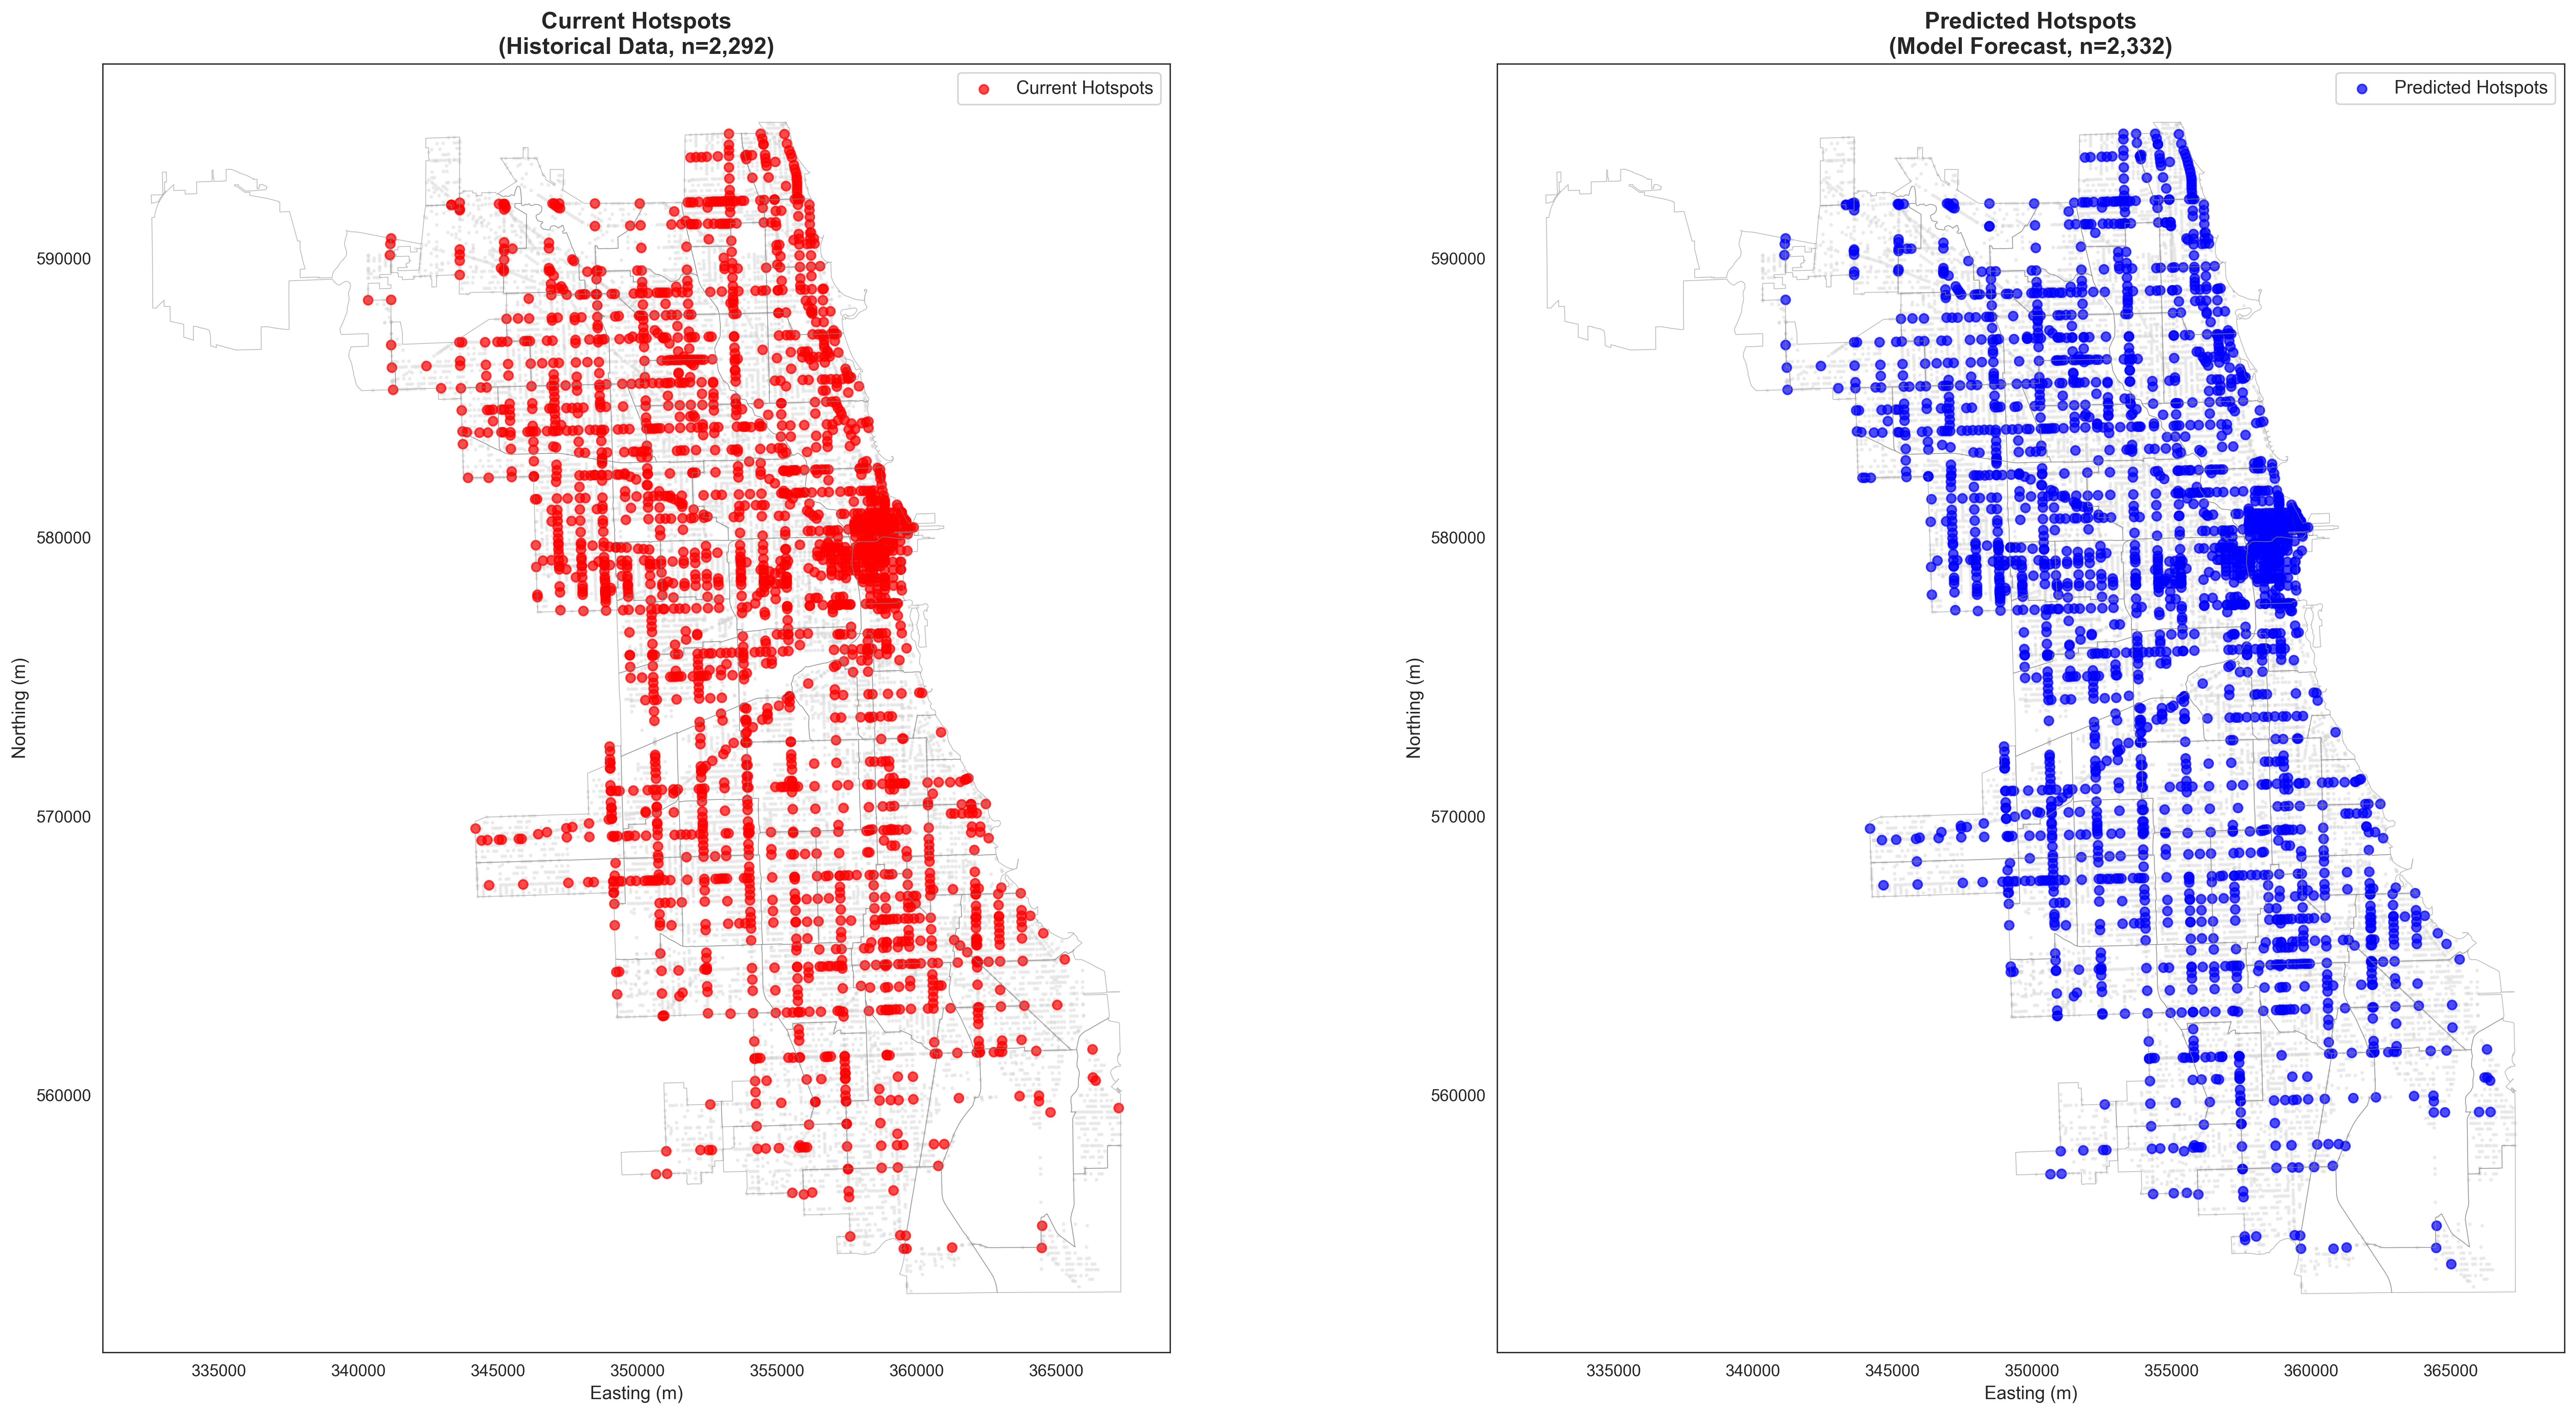
\includegraphics[width=0.45\textwidth]{map_comparison_current_vs_predicted.png}
    \caption{Side-by-side comparison of (a) current hotspots from historical data (2,292 intersections) and (b) predicted future hotspots from Gradient Boosting model (2,332 intersections), demonstrating high spatial stability with 1,875 persistent hotspots (80.8\% overlap) and 457 newly emerging high-risk areas.}
    \label{fig:hotspot_comparison}
\end{figure}

\begin{figure}[t]
    \centering
    \includegraphics[width=0.45\textwidth]{map_community_choropleth.png}
    \caption{Community-level choropleth maps showing (a) total crashes by community area revealing concentration in downtown and major corridors, and (b) crash rate per 1,000 population revealing disparities: Near West Side (1,168 crashes/1k), West Town (969/1k), and Austin (940/1k) experience highest per-capita rates.}
    \label{fig:community_choropleth}
\end{figure}

\section{Discussion}

\subsection{Interpretation of Predictive Results}

Our Gradient Boosting model achieved strong predictive performance (PR-AUC=0.772, ROC-AUC=0.946), demonstrating that machine learning can effectively identify future crash hotspots. The dominance of historical crash count (90\% feature importance) indicates strong temporal persistence—locations with frequent past crashes remain high-risk without intervention. This justifies proactive, data-driven infrastructure improvements. Network centrality (2.3\%) confirms that road structure influences crash risk beyond traffic volume.

\subsection{Inequality and Environmental Justice}

Our analysis revealed a critical disparity: while overall crash rates show no clear income gradient, \textbf{severe injury rates are 80\% higher in low-income communities} (Q1: 1.8\% vs Q4: 1.0\%, r=-0.488, p<0.001). This inequality of outcomes may stem from older vehicles lacking safety features, poor road infrastructure, longer EMS response times, or greater pedestrian/cyclist exposure. These findings align with environmental justice frameworks \cite{bullard2007growing}, suggesting that Vision Zero initiatives should prioritize communities with high severe injury rates.

\subsection{Spatial Clustering Implications}

The significant positive spatial autocorrelation (Moran's I=0.161, p<0.001) confirms crashes cluster geographically. This justifies: (1) targeted interventions in High-High cluster zones (964 intersections, 5\% of total), (2) recognizing spillover effects between neighboring intersections, and (3) corridor-level interventions on major arterials.

\subsection{Policy Recommendations and Limitations}

\textbf{Immediate Priorities}: Deploy engineering improvements at 1,875 persistent hotspots (protected turns, pedestrian islands, red-light cameras), focusing on Near North Side, Loop, and Near West Side. \textbf{Proactive Measures}: Monitor 457 emerging hotspots with enforcement and temporary calming. \textbf{Equity Focus}: Prioritize severe-injury-reduction in Q1 communities, invest in pedestrian/cycling infrastructure in low-vehicle-ownership areas.

\textbf{Limitations}: The model's reliance on historical crashes (90\% importance) may perpetuate existing patterns. Crash data reflects police-reported incidents, potentially undercounting minor crashes. We assume temporal stationarity, though structural changes (COVID-19, micromobility) may alter relationships. Intersection-level aggregation masks within-intersection heterogeneity. Weather, construction, and real-time traffic are omitted. Despite limitations, temporal validation ensures realistic performance estimates.

\subsection{Ethical Considerations}

Traffic safety algorithms raise important ethical questions. \textbf{Fairness}: Predictive models risk reinforcing inequalities if interventions follow predictions that undercount crashes in underserved areas—we mitigate this by explicit inequality analysis and equity-focused prioritization. \textbf{Privacy}: While using aggregated data, fine-grained models could enable surveillance or discriminatory insurance pricing. \textbf{Accountability}: Automated resource allocation requires transparency and public input—algorithms should not replace community engagement. \textbf{Resource allocation}: Identifying hotspots implicitly de-prioritizes other locations; cities must balance data-driven targeting with baseline safety investments. Our open-source approach promotes transparency and stakeholder auditing.

\section{Conclusion}

This study demonstrates that machine learning, network science, and spatial statistics can effectively predict traffic crash hotspots and quantify inequality in crash exposure across urban neighborhoods. Our temporally-validated Gradient Boosting model achieved PR-AUC of 0.772, successfully identifying future hotspots at 19,200 Chicago intersections. We confirmed significant spatial clustering (Moran's I=0.161) and identified 964 High-High cluster intersections requiring intervention. Critically, we documented substantial inequality in severe injury rates, with low-income communities experiencing 80\% higher rates than affluent areas.

These findings have direct policy implications: (1) prioritize infrastructure improvements at 1,875 persistent hotspots, (2) proactively monitor 457 emerging hotspots, and (3) implement equity-focused severe-injury-reduction programs in low-income communities. By integrating predictive modeling with inequality analysis and spatial clustering, we provide a comprehensive framework for data-driven, equitable urban traffic safety policy.

Future work should incorporate real-time traffic data, explore causal inference methods to isolate intervention effects, and extend the analysis to other cities to test generalizability. Deep learning approaches (e.g., graph neural networks on road networks, recurrent models for temporal dynamics) may further improve prediction accuracy. Ultimately, this research demonstrates the potential of urban computing to advance both public safety and social equity in cities.

\section{Acknowledgements}

We thank the City of Chicago for providing open access to traffic crash data through the Chicago Data Portal. We are grateful to OpenStreetMap contributors for maintaining the road network data. This work benefited from computational resources provided by Virginia Tech. We thank Professor Naren Ramakrishnan for guidance on urban computing methodologies and feedback on the project design. We acknowledge the U.S. Census Bureau for providing demographic data through the American Community Survey.

\section{Author Contributions}

All authors contributed equally to this project. Specific contributions:

\textbf{Shubam Khantwal}: Led data preprocessing pipeline development, implemented spatial matching algorithms for crash-to-intersection linkage, computed network centrality measures using OSMnx and NetworkX, conducted exploratory data analysis, and contributed to manuscript writing.

\textbf{Siddarth Bandi}: Designed and implemented temporal validation framework, developed machine learning models (Logistic Regression, Random Forest, Gradient Boosting), performed feature importance analysis, created model evaluation visualizations, and led manuscript writing and editing.

\textbf{Venkata Sai Yaswanth Madiraju}: Conducted inequality analysis across income quartiles, performed statistical hypothesis testing, implemented spatial autocorrelation analysis (Moran's I and LISA), created geographic visualizations and choropleth maps, and contributed to manuscript writing.

All authors jointly designed the study, interpreted results, and reviewed the final manuscript.

\section{Data and Code Availability}

All code, datasets, and analysis notebooks are available in our GitHub repository:

\url{https://github.com/siddarthx07/Crash-Inequality-Chicago}

The repository includes:
\begin{itemize}
    \item Data preprocessing scripts (\texttt{scripts/} directory)
    \item Jupyter notebooks for analysis (\texttt{notebooks/} directory)
    \item Trained model files (\texttt{models/} directory)
    \item Generated results and figures (\texttt{results/} directory)
    \item Requirements file for reproducing the Python environment
\end{itemize}

Raw data sources:
\begin{itemize}
    \item Chicago Traffic Crashes: \url{https://data.cityofchicago.org/Transportation/Traffic-Crashes-Crashes/}
    \item Chicago Community Areas: \url{https://data.cityofchicago.org/Facilities-Geographic-Boundaries/Boundaries-Community-Areas/}
    \item OpenStreetMap: Downloaded via OSMnx Python library
    \item U.S. Census ACS: \url{https://data.census.gov/}
\end{itemize}

\begin{thebibliography}{99}

\bibitem{nhtsa2021}
National Highway Traffic Safety Administration, "Traffic Safety Facts 2021," U.S. Department of Transportation, 2022.

\bibitem{chen2016crash}
C. Chen, G. Zhang, R. Tarefder, J. Ma, H. Wei, and H. Guan, "A multinomial logit model-Bayesian network hybrid approach for driver injury severity analyses in rear-end crashes," \textit{Accident Analysis \& Prevention}, vol. 80, pp. 76-88, 2015.

\bibitem{gutierrez2020modern}
C. Gutierrez-Osorio and C. Pedraza, "Modern data sources and techniques for analysis and forecast of road accidents: A review," \textit{Journal of Traffic and Transportation Engineering}, vol. 7, no. 4, pp. 432-446, 2020.

\bibitem{bao2020spatial}
J. Bao, P. Liu, and S. V. Ukkusuri, "A spatiotemporal deep learning approach for citywide short-term crash risk prediction with multi-source data," \textit{Accident Analysis \& Prevention}, vol. 122, pp. 239-254, 2019.

\bibitem{plug2011spatial}
C. Plug, J. Xia, and C. Caulfield, "Spatial and temporal visualisation techniques for crash analysis," \textit{Accident Analysis \& Prevention}, vol. 43, no. 6, pp. 1937-1946, 2011.

\bibitem{prasannakumar2011spatial}
V. Prasannakumar, H. Vijith, R. Charutha, and N. Geetha, "Spatio-temporal clustering of road accidents: GIS based analysis and assessment," \textit{Procedia-Social and Behavioral Sciences}, vol. 21, pp. 317-325, 2011.

\bibitem{anselin1995local}
L. Anselin, "Local indicators of spatial association—LISA," \textit{Geographical Analysis}, vol. 27, no. 2, pp. 93-115, 1995.

\bibitem{jacquez2005spatial}
G. M. Jacquez, "Spatial cluster analysis," in \textit{The Handbook of Geographic Information Science}, 2005, pp. 395-416.

\bibitem{xu2013network}
C. Xu, W. Wang, and P. Liu, "A genetic programming model for real-time crash prediction on freeways," \textit{IEEE Transactions on Intelligent Transportation Systems}, vol. 14, no. 2, pp. 574-586, 2013.

\bibitem{kerner2015traffic}
B. S. Kerner, \textit{Introduction to Modern Traffic Flow Theory and Control: The Long Road to Three-Phase Traffic Theory}. Springer, 2009.

\bibitem{cottrill2010evaluating}
C. D. Cottrill and P. Thakuriah, "Evaluating pedestrian crashes in areas with high low-income or minority populations," \textit{Accident Analysis \& Prevention}, vol. 42, no. 6, pp. 1718-1728, 2010.

\bibitem{beck2007motor}
L. F. Beck, A. M. Dellinger, and M. E. O'Neil, "Motor vehicle crash injury rates by mode of travel, United States: using exposure-based methods to quantify differences," \textit{American Journal of Epidemiology}, vol. 166, no. 2, pp. 212-218, 2007.

\bibitem{bullard2007growing}
R. D. Bullard, \textit{Growing Smarter: Achieving Livable Communities, Environmental Justice, and Regional Equity}. MIT Press, 2007.

\end{thebibliography}

\end{document}

